\subsection{Layer Software Dependencies}
The entire front-end will depend on Bootstrap and the React library. The front-end will also depend on a consistent connection to the Query Manager on the Server layer.

\subsection{Login Subsystem}
The Login Subsystem will provide an interface for users to login into the application. Users will be able to log in with their Google accounts.


\begin{figure}[h!]
	\centering
 	
\includegraphics[width=0.60\textwidth]{images/login}
 \caption{Login Subsystem diagram}
\end{figure}

\subsubsection{Subsystem Software Dependencies}
For a user to log in with their Google accounts, the Login Subsystem will depend on the GoogleLogin library.

\subsubsection{Subsystem Programming Languages}
The Login Subsystem will be developed using, React.js, HTML, and CSS.

\subsubsection{Subsystem Data Processing}
When the user logs in with their Google account, they will select the Google login button. The Login Subsystem will then call on the GoogleLogin API which users will log in with. If the login is successful, the Login Subsystem will redirect the user to the Home Page. If the login fails, the user will be given an error message and prompted to re-enter their credentials.

%------------> Shopping List
\subsection{Shopping List Subsystem}
The Shopping List Subsystem will provide an interface for users to view all the items on their current shopping list. It will also allow users to add and remove items.

\begin{figure}[h!]
	\centering
 	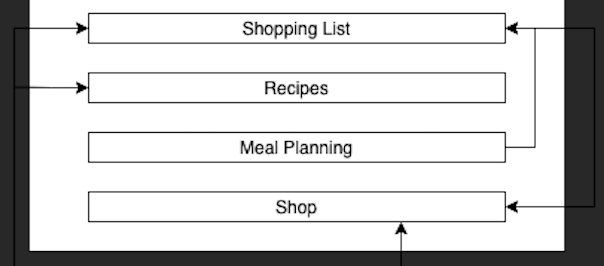
\includegraphics[width=0.60\textwidth]{images/shoppingList}
 \caption{Shopping List Subsystem diagram}
\end{figure}

\subsubsection{Subsystem Software Dependencies}
The Shopping List Subsystem has no additional dependencies.

\subsubsection{Subsystem Programming Languages}
The Shopping List Subsystem will be developed using, React.js, HTML, and CSS.

\subsubsection{Subsystem Data Processing}
The Shopping List Subsystem will retrieve the current user's shopping list from the Query Manager and display all relevant information.

%------------> Recipes
\subsection{Recipes Subsystem}
The Recipes Subsystem will provide an interface for users to view and shop for all recipes in the system's database. It will also allow users to create and edit their recipes.

\begin{figure}[h!]
	\centering
 	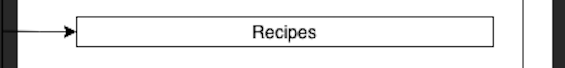
\includegraphics[width=0.60\textwidth]{images/recipes}
 \caption{Recipes Subsystem diagram}
\end{figure}

\subsubsection{Subsystem Software Dependencies}
The Recipes Subsystem has no additional dependencies.

\subsubsection{Subsystem Programming Languages}
The Recipes Subsystem will be developed using, React.js, HTML, and CSS.

\subsubsection{Subsystem Data Processing}
The Recipes Subsystem will display all recipes retrieved by the Query Manager.

%------------> Meal Plan
\subsection{Meal Plan Subsystem}
The Meal Plan Subsystem will provide an interface for users to view and edit their Meal Plans.

\begin{figure}[h!]
	\centering
 	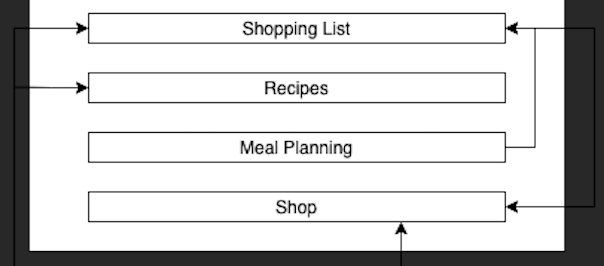
\includegraphics[width=0.60\textwidth]{images/shoppingList}
 \caption{Meal Plan Subsystem diagram}
\end{figure}

\subsubsection{Subsystem Software Dependencies}
The Meal Plan Subsystem has no additional dependencies.

\subsubsection{Subsystem Programming Languages}
The Meal Plan Subsystem will be developed using, React.js, HTML, and CSS.

\subsubsection{Subsystem Data Processing}
The Meal Plan Subsystem will display the current user's Meal Plans that are retrieved by the Query Manager.

%------------> Shop
\subsection{Shop Subsystem}
The Shop Subsystem will provide an interface for users to view the results of the shopping trip being planned.

\begin{figure}[h!]
	\centering
 	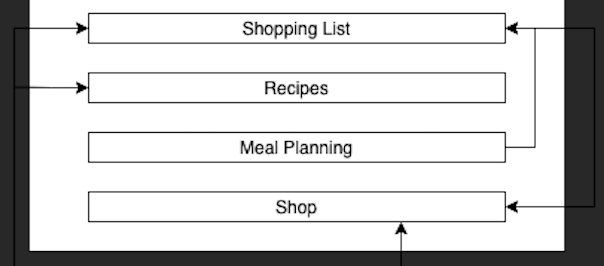
\includegraphics[width=0.60\textwidth]{images/shoppingList}
 \caption{Shop Subsystem diagram}
\end{figure}

\subsubsection{Subsystem Software Dependencies}
The Shop Subsystem depends on a consistent connection to the Shop Manager on the Server layer.

\subsubsection{Subsystem Programming Languages}
The Shop Subsystem will be developed using, React.js, HTML, and CSS.

\subsubsection{Subsystem Data Processing}
The Shop Subsystem will display all information that is calculated by the Shopping Manager.


